\documentclass[11pt,oneside]{book}
\usepackage[english, italian]{babel} 
\usepackage{microtype}
\usepackage[utf8]{inputenc}
\usepackage{subfigure}
\usepackage{epsfig}
\usepackage{amsmath, amssymb}
\usepackage[linesnumbered,lined,commentsnumbered,italiano]{algorithm2e}
\usepackage{fancybox}
\usepackage{listings}
\usepackage{url}
\usepackage{graphicx}
\usepackage{todonotes}
\usepackage{moreverb}
\usepackage{float}
\usepackage[labelfont=it,textfont={it}]{caption}
\usepackage[final,bookmarks,breaklinks,colorlinks,allcolors=black]{hyperref}
\usepackage{color}
\usepackage[block=ragged,backend=biber,natbib=true]{biblatex} % Use the bibtex backend with the authoryear citation style (which resembles APA)
\addbibresource{bibliography.bib} % The filename of the bibliography
\usepackage[autostyle=true]{csquotes}
\usepackage{xcolor} % Required to generate language-dependent quotes in the bibliography

%%%%%%%%%%%%%%%%%%%%%%%%%%%%
\definecolor{mygreen}{rgb}{0,0.6,0}
\definecolor{mygray}{rgb}{0.5,0.5,0.5}
\definecolor{mymauve}{rgb}{0.58,0,0.82}
\lstset{ %
	backgroundcolor=\color{white},   % choose the background color; you must add \usepackage{color} or \usepackage{xcolor}; should come as last argument
	basicstyle=\footnotesize,        % the size of the fonts that are used for the code
	breakatwhitespace=false,         % sets if automatic breaks should only happen at whitespace
	breaklines=true,                 % sets automatic line breaking
	captionpos=b,                    % sets the caption-position to bottom
	commentstyle=\color{mygreen},    % comment style
	deletekeywords={...},            % if you want to delete keywords from the given language
	escapeinside={\%*}{*)},          % if you want to add LaTeX within your code
	extendedchars=true,              % lets you use non-ASCII characters; for 8-bits encodings only, does not work with UTF-8
	frame=single,
	keepspaces=true,                 % keeps spaces in text, useful for keeping indentation of code (possibly needs columns=flexible)
	keywordstyle=\color{blue},       % keyword style
	morekeywords={*,...},            % if you want to add more keywords to the set
	numbers=left,                    % where to put the line-numbers; possible values are (none, left, right)
	numberstyle=\tiny\color{mygray}, % the style that is used for the line-numbers
	rulecolor=\color{black},         % if not set, the frame-color may be changed on line-breaks within not-black text (e.g. comments (green here))
	showspaces=false,                % show spaces everywhere adding particular underscores; it overrides 'showstringspaces'
	showstringspaces=false,          % underline spaces within strings only
	showtabs=false,                  % show tabs within strings adding particular underscores
	stringstyle=\color{mymauve},     % string literal style
	tabsize=2,	                   % sets default tabsize to 2 spaces
	title=\lstname                   % show the filename of files included with \lstinputlisting; also try caption instead of title
}
%%%%%%%%%%%%%
\definecolor{gray}{rgb}{0.4,0.4,0.4}
\definecolor{darkblue}{rgb}{0.0,0.0,0.6}
\definecolor{cyan}{rgb}{0.0,0.6,0.6}


\definecolor{javared}{rgb}{0.6,0,0} % for strings
\definecolor{javagreen}{rgb}{0.25,0.5,0.35} % comments
\definecolor{javapurple}{rgb}{0.5,0,0.35} % keywords
\definecolor{javadocblue}{rgb}{0.25,0.35,0.75} % javadoc

\lstdefinelanguage{FLY}
{
  morestring=[b]",
  morecomment=[l]{//},
  morecomment=[s]{/}{/},
  identifierstyle=\color{black},
  keywordstyle=\color{javapurple},
  morekeywords={func,var,while, if, then, else,for, in, println, fly ,on,thenall,as,then,require,native}% list your attributes here
}

\lstset{language=FLY,
basicstyle=\ttfamily\scriptsize,
keywordstyle=\color{javapurple}\bfseries,
stringstyle=\color{javared},
commentstyle=\color{javagreen},
morecomment=[s][\color{javadocblue}]{/*}{/},
numbers=left,
numberstyle=\tiny\color{black},
stepnumber=1,
numbersep=10pt,
tabsize=4,
showspaces=false,
showstringspaces=false}
%%%%%%%%%%%%%%%%%%%%%%%%
\begin{document}
\selectlanguage{italian}

\begin{titlepage}
\begin{center}

\epsfig{file=Figure/logo_standard.jpg,width=2.5truecm}\\[0.2truecm]
{\Large Universit\`a degli Studi di Salerno}\\[0.2truecm]
{\large Dipartimento di Informatica}\\
\hrulefill
\vfill
{\large Tesi di Laurea di I livello in }\\[0.2truecm]
{\Large Informatica}\\
\vfill\vfill
{\Huge Implementazione di un ambiente di esecuzione basato su Kubernetes nel linguaggio FLY}
\vfill\vfill


{\bf Relatore} \hfill {\bf Candidato}\ \ \\
Prof. Vittorio Scarano \hfill Luigi Barbato\\
{\bf Correlatore} \hfill {\bf }\ \ \\
Dott. Giuseppe D'Ambrosio \hfill \ \ \\
Dott. Carmine Spagnuolo \hfill \ \ \\

\vfill
\hrulefill 

Anno Accademico 2020-2021

\end{center}
\end{titlepage}

\pagenumbering{roman}
\chapter*{Abstract}
% Il Cloud Computing si è ormai affermato come paradigma fondante per la costruzione di infrastrutture di calcolo grazie alla possibilità di ottenere risorse di computazione sotto forma di servizi. Un mercato inizialmente composto da pochi Cloud provider conta ormai la presenza di numerosi di concorrenti, ognuno con la propria piattaforma e le proprie soluzioni. La volontà di sfruttare questa varietà di provider ha portato alla nascita del multi-cloud, ovvero l’utilizzo di più ambienti Cloud compresi in una singola architettura per ottenere maggiore affidabilità, un miglior rapporto qualità-prezzo e riducendo la dipendenza dal singolo. Tuttavia la forte diversità tra le API fornite per l'accesso ai vari servizi rende l'introduzione del multi-cloud particolarmente complessa per cui vi è la necessità di strumenti che ne facilitino l'utilizzo. È in questo ambito che nasce Fly, un Domain-Specific Language per il calcolo scientifico su multi-cloud il cui obiettivo è quello di semplificare lo sviluppo di applicazioni su Cloud introducendo un livello di astrazione aggiuntivo grazie al quale l'utente non necessita di conoscere le specifiche API del provider che vuole utilizzare. L'obiettivo di questo lavoro di tesi è di presentare due importanti funzionalità introdotte all'interno di Fly, ovvero la possibilità di utilizzare un ambiente di debug e il supporto alle sorgenti dati esterne. È infatti importante fornire un ambiente indipendente dal Cloud ma che ne simuli fedelmente il comportamento, in quanto lo sviluppo di applicazioni comprende l'esecuzione di numerosi test per verificarne il funzionamento, tuttavia eseguirli su Cloud comporta dei costi sia in tempo che in denaro. La soluzione sviluppata sfrutta LocalStack, un framework che consente di creare un ambiente AWS in locale completo di tutti i suoi servizi che l’utente può utilizzare come ambiente di test allo stesso modo di un ambiente su Cloud. La seconda parte della tesi riguarda il supporto alle sorgenti dati esterne, in particolare la possibilità di utilizzare all'interno dei programmi Fly sia file dati strutturati che database relazionali, siano essi in locale o su Cloud. In particolare vengono introdotti metodi per la gestione dei file e  dei database MySQL che comprendono il supporto alle query. L'implementazione di database su Cloud è possibile mediante il modello Database as a Service (DBaaS), in particolare Amazon Web Services offre il servizio Amazon RDS mentre Microsoft Azure mette a disposizione il servizio Azure for MySQL. Entrambi sono implementati all'interno di Fly utilizzando le soluzioni e gli strumenti più validi in base al contesto, sfruttando il grande vantaggio del modello DBaaS che consente di accedere ai database su Cloud allo stesso modo di come si farebbe con database locali.

Negli ultimi anni, il paradigma del Cloud Computing ha ottenuto grande successo grazie ai numerosi vantaggi che esso offre.
I motivi del suo successo sono ampliamente giustificati dal grande numero di vantaggi che ha portato. 
Tra questi, il più importante consiste nella possibilità di accedere a diversi tipi di risorse hardware e software mediante un paradigma
basato sui servizi. 
Kubernetes è una piattaforma portatile, estensibile e open-source per la gestione e l'orchestrazione di applicativi Cloud-Native,
ovvero applicativi svilluppati appositamente per essere utilizzati in ambienti Cloud. 
Esso consente di orchestrare applicazioni containerizzate all'interno di cluster di nodi su cui vengono eseguiti, grazie agli strumenti ed alle API fornite, operazioni per la gestione del carico di lavoro, 
del traffico di rete e dell'archiviazione. 
Nonostante i vantaggi, Kubernetes rimane un sistema estremamente complesso ed articolato da utilizzare, necessitando di conoscenze specifiche per essere usato in modo efficace.
Fly è un Domain-Specific Language per il calcolo scientifico su multi-cloud il cui obiettivo è quello di semplificare lo sviluppo di applicazioni su Cloud introducendo un livello di astrazione
che permetta all'utente di utilizzare le funzionalità e le potenzialità di un ambiente cloud in modo semplice ed efficiente. 
Questo lavoro di tesi presenta l'integrazione di un ambiente di esecuzione basato su Kubernetes all'interno del linguaggio di programmazione Fly. 
Grazie ai costrutti specifici introdotti all'interno del linguaggio FLY è possibile automatizzare completamente il processo di esecuzione di un'applicazione su Kubernetes.

\vfill
\centerline{\Large\sf Questa tesi è stata sviluppata in  \raisebox{-0.05truecm}{
\epsfig{file=Figure/logo_small.jpg,width=2truecm}}}

\tableofcontents
\pagestyle{plain}

%%%%%%%%%%%%%%%%%%%%%%%%%%%%
\chapter{Introduzione}
\setcounter{page}{1} 	% devono seguire solo il primo capitolo
\pagenumbering{arabic}	% devono seguire solo il primo capitolo
\section{Cloud Computing}
\subsection{Panoramica}
Il Cloud Computing è una particolare ed innovativa forma di erogazione di risorse da un fornitore ad un cliente attraverso la rete internet. Esso segue un paradigma architetturale di tipo distribuito ed i servizi offerti possono essere vari come l'archiviazione, la computazione oppure una semplice trasmissione dati.
Le risorse e le configurazioni a cui fa fede, non sono predefinite ma, con l'utilizzo di processi automatizzati, ogni
%Approssimativo perchè esiste anche la possibilità di crearsi la propria infrastruttura cloud%
 Cloud Provider è in grado di personalizzare e scalare le risorse opportune per quel determinato servizio a quel determinato cliente. Una volta che quest'ultimo termina l'utilizzo delle risorse assegnate, queste tornano nuovamente disponibili, pronte per una nuova assegnazione.

\subsection{Vantaggi}
E' possibile individuare i maggiori vantaggi che motivano le aziende e gli sviluppatori a utilizzare il Cloud Computing per i propri applicativi o per le proprie infrastrutture.
%In realtà non è del tutto corretto perchè l'azienda può scegliere di costruirsi la propria infrastruttura su un Cloud locale%
\subsubsection{Costi}
E' chiaro che in quest'ottica, il modello economico Pay-as-you-go è diventato parte integrante della strategia di fruizione dei servizi, in quanto porta innumerevoli vantaggi ai fornitori ma sopratutto ai clienti stessi, tra cui:
    \begin{itemize}
    \item \textbf{Ottimizzazione del capitale} - la libertà di pagare solo ciò di cui si ha realmente bisogno, l'eliminazione dei costi di investimento e dei costi di mantenimento ed il miglioramento dell'efficienza energetica permettono un notevole abbattimento dei costi ed un'ottimizzazione del capitale.
    \item \textbf{Flessibilità} - I clienti, in ogni momento ed in maniera quasi istantanea, hanno la massima libertà di poter annullare, sostituire o fermare qualsiasi servizio in corso.
    \item \textbf{Scalabilità} - Il sistema adottato, accompagna senza problemi la crescita di piccole infrastrutture. In effetti, per una Start-up agli inizi, è pratico dotarsi di uno strumento adeguato in termini di prezzi e funzionalità, per poi farlo crescere in parallelo con l'evoluzione e le ambizioni dell'azienda.
    \end{itemize}

\subsubsection{Performance e scalabilità}
La tecnologia alla base del Cloud Computing è la virtualizzazione la quale, date le sue potenzialità, permette di ridimensionare agilmente le risorse assegnate. La potenza computazionale, la larghezza di banda e lo spazio di archiviazione sono esempi di risorse che possono essere scalate in base al carico di richieste, andando quindi ad allocarne una quantità maggiore in caso di maggiore attività, una quantità minore in caso di minore attività e a deallocare quelle inutilizzate in caso d'inattività prolungata.

\subsection{Modelli di servizio}
Il Cloud Computing è un mondo in continua crescita ed evoluzione, nuovi prodotti e servizi cloud arrivano quasi ogni giorno, spinti dalle costanti innovazioni tecnologiche.
Nonostante la maturità del mercato, molte organizzazioni non sono ancora a conoscenza dei servizi e dei modelli d'implementazione che i diversi Cloud Provider forniscono.
I tre modelli principali a oggi maggiormente diffusi sono così definiti:

\subsubsection{Software as a Service (Saas)}
Software as a Service (SaaS) è il modello di servizio cloud che fornisce l'accesso a un prodotto software completo, eseguito e gestito dal fornitore del servizio.
In questo particolare modello, il fornitore ha la piena responsabilità sull'intero ciclo di vita del software e sulla manutenzione dell'infrastruttura sottostante. Questo consente al cliente di concentrarsi esclusivamente su come utilizzare al meglio le specifiche e le funzionalità del software offerto.

\subsubsection{Platform as a Service (Saas)}
Platform as a Service (PaaS) è il modello usato più comunemente per lo sviluppo di applicazioni. Il fornitore del servizio fornisce l'accesso alle proprie risorse infrastrutturali come: basi di dati, sistemi operativi e server, senza la complessità di gestione che ne deriva. Questo permette al cliente di dedicare le proprie risorse all'ottimizzazione dell'applicativo invece che all'installazione e alla configurazione dell'infrastruttura.

\subsubsection{Infrastructure as a Service (Saas)}
Infrastructure as a Service (IaaS) è il modello che permette al cliente d'implementare la propria infrastruttura cloud. Il Cloud Provider fornisce l'accesso on-demand delle proprie risorse (sia fisiche che virtuali) volte alla computazione, archiviazione e alla rete.
Il cliente ottiene così l'enorme vantaggio di poter distribuire e gestire i propri applicativi avendo la sicurezza di avere risorse sempre disponibili, affidabili e scalabili.

\subsection{Modelli di distribuzione}
Ogni modello d'implementazione del cloud ha una propria configurazione unica con una gamma di requisiti diversi e vantaggi associati.

\subsubsection{Public Cloud}
Il Public Cloud è un modello di distribuzione in cui i servizi cloud sono di proprietà di fornitori esterni. Scegliere questa metodologia garantisce una maggiore agilità operativa e una scalabilità pressoché illimitata, perché sfrutta le funzionalità e le risorse di grandi fornitori come Google, Microsoft e Amazon.
Trattandosi inoltre di ambienti gestiti, il cliente si solleva dalle responsabilità di manutenzione e controllo delle risorse utilizzate.

\subsubsection{Private Cloud}
Nel modello di distribuzione Private Cloud si sceglie di sviluppare, mantenere e gestire la propria infrastruttura cloud, fornendo l'accesso solo alla propria rete interna. Con il Private Cloud le organizzazioni mantengono un controllo completo dell'infrastruttura. Questo si traduce in un controllo completo delle proprie risorse e ad una maggior libertà di personalizzazione dei servizi, che sono consumati all'interno del cloud.

\subsubsection{Hybrid Cloud}
L’Hybrid Cloud è un modello di distribuzione ibrido in quanto 
Si sceglie di unire i vantaggi del cloud pubblico e di quello privato.
Ad esempio, si possono utilizzare le risorse del Public Cloud per attività di computazione, e tenere al sicuro i dati sensibili e le applicazioni critiche nel Private Cloud. Oppure, di fronte a picchi improvvisi e temporanei della domanda di risorse, le organizzazioni possono scegliere di spostare i carichi di lavoro dal Private Cloud al Public Cloud.
Utilizzato in questo modo, l’Hybrid Cloud consente di ottenere il meglio da entrambe le infrastrutture.
%!TEX root = ../../00main.tex

\section{Multi-cloud}
il successo del cloud computing ha portato alla nascita di molteplici Cloud Provider. Questo ha spinto gli sviluppatori a sfruttare diversi cloud provider nella stessa architettura portando alla nascita del multi-cloud
Il multi-cloud è una forma architetturale in cui si utilizzano risorse e servizi di Cloud Provider differenti convergendoli in una singola architettura eterogenea. 
Le motivazioni che muovono un'organizzazione ad adottare questo tipo di strategia sono varie:
\begin{itemize}
\item \textbf{Maggiore flessibilità} - Ogni Cloud Provider propone la propria gamma di servizi che differiscono tra loro in caratteristiche diventando migliori da utilizzare per particolari situazioni rispetto che altre. La possibilità e quindi la libertà di poter scegliere e selezionare distintamente i singoli servizi concedono all'utente il vantaggio di poter coprire totalmente le proprie esigenze.
\item \textbf{Localizzazione} - Ogni Cloud Provider detiene le proprie infrastrutture dislocate in diverse aree geografiche, l'utente può decidere di utilizzarle in base alle proprie esigenze logistiche e legali.
\item \textbf{Prestazioni} - L'utilizzo di risorse provenienti da fornitori distinti, permette una distribuzione più ampia dei servizi dell'applicativo.
\end{itemize}
%!TEX root = ../../00main.tex

\section{Containerizzazione}
La virtualizzazione è una tecnologia che permette di mettere a disposizione risorse hardware come CPU e memoria sottoforma di risorse virtuali. Attraverso la virtualizzazione è possibile utilizzare delle risorse virtuali allo stesso modo di come si farebbe con delle risorse fisiche permettendo di migliorare la scalabilità e i carichi di lavoro, usando al contempo un minor numero di macchine, una quantità di energia elettrica ridotta, generando così un risparmio sui costi di infrastruttura e gestione.
Uno dei principali vantaggi della virtualizzazione è la razionalizzazione e l'ottimizzazione delle risorse hardware in quanto più macchine virtuali possono girare contemporaneamente su un sistema fisico condividendo le risorse della piattaforma.
La metodologia più semplice di virtualizzazione prevede la creazione di una macchina virtuale che va a simulare un'intero sistema fisico con risorse come CPU, memoria e componenti di reti. Una macchina virtuale dovrà quindi essere utilizzata come un normale computer desktop, eseguendo un proprio sistema operativo e rimanendo completamente isolata dall'hardware fisico sottostante.
Con il termine containerizzazione si intende una para-virtualizzazione dell'ambiente applicativo che consente di eseguire software, librerie, dipendenze e tutte le componenti necessarie, in un processo isolato che prende il nome di contenitore. Esso può essere considerato un vero e proprio eseguibile che non dipende da alcuna sorgente esterna. Questo lo rende estremamente portatile e affidabile in quanto può essere eseguito e trasferito in ogni tipo di ambiente e d'infrastruttura.
L'idea alla base del paradigma non è in realtà nuova in quanto sfrutta una funzionalità del kernel Linux presente già dalla versione 2.6.24 che permette l'isolamento e la gestione delle risorse di uno o più processi.

\subsection{Vantaggi}
Il grande successo della virtualizzazione basata su container deriva dai grandi vantaggi che essa garantisce. Tra essi troviamo:
\begin{itemize}
\item \textbf{Portabilità} - I container sono altamente portabili in quanto contengono al loro interno tutte le dipendenze e le componenti necessarie all'esecuzione dell'applicazione, evitando così problemi di compatibilità
\item \textbf{Efficienza} - I container hanno la capacità di condividere il kernel della macchina ospitante evitando così di dover disporre di risorse hardware e software dedicate. Inoltre è sempre possibile aumentare e diminuire le risorse in modo istantaneo, in base alle proprie esigenze, in modo da non incorrere in sprechi o in carenze.
\item \textbf{Ottimizzazione dello spazio} - L'immagine dell'applicazione che viene eseguita all'interno del contenitore, incapsula solo ed unicamente le componenti e le informazioni necessarie alla sua esecuzione.
\end{itemize}
\section{Docker}
Docker è una tecnologia open–source per la costruzione, spostamento, distribuzione e rilascio di
applicazioni basate su container, distribuita sotto Licenza Apache Common 2.0, disponibile per
tutte le maggiori piattaforme in grado di eseguire container in ambienti Linux oppure Windows.
La struttura stessa dei container garantisce il loro isolamento, permettendo l’esecuzione multipla
su un singolo host, sfruttando direttamente il kernel della macchina senza la necessità di un server
hypervisor. In questo modo, i container sono il centro dello sviluppo dell’applicazione, la quale
viene costruita come insieme di container per esprimere le dipendenze, permettendone una facile
distribuzione e testing in ambienti diversi, fino alla messa in campo in produzione in un data
center locale, presso un cloud provider o una soluzione ibrida tra le precedenti.
Docker utilizza e crea differenti tipi di oggetti, come immagini e container. Un container costituisce 
un’istanza di un’immagine in esecuzione, con il quale è possibile interagire direttamente dalla
macchina host, e può essere visto come un’evoluzione di un processo, isolato dagli altri container
e dal sistema host.
Un’immagine, invece, costituisce un template di sola lettura, utilizzato per la creazione di un
container Docker. Solitamente, un’immagine viene costruita sulla base di un’altra immagine alla
quale vengono aggiunte le configurazioni necessarie e peculiari dell’applicazione. La definizione
di un’immagine avviene all’interno di un file, chiamato Dockerfile, nel quale vengono indicate
le istruzioni, ognuna delle quali aggiunge un layer all’interno dell’immagine finale, in modo tale
che, di volta in volta, vengano ricompilati solo gli strati che effettivamente sono stati modificati.
%!TEX root = ../../00main.tex

\section{Kubernetes}
Kubernetes è una piattaforma portatile, estensibile e open-source per la gestione e l'orchestrazione di applicativi Cloud-Native.
La piattaforma è scritta in linguaggio Go ed è stato inizialmente sviluppato da Google per migliorare la gestione dei propri applicativi. Il progetto è attualmente parte della Cloud Native Computing Foundation\footnote{Cloud Native Computing Foundation - \url{https://www.cncf.io/}}, organizzazione che promuove e mantiene progetti open-source volti all'approccio Cloud Native.
Kubernetes utilizza un insieme di oggetti fruibili tramite API per descrivere lo stato desiderato del cluster, indicando, ad esempio, quali applicazioni eseguire, quali immagini utilizzare, il numero di repliche da istanziare, quali risorse di rete e di spazio su disco rendere disponibili. L'interazione viene resa possibile grazie a kube-apiserver, il server HTTP che implementa l'API Kubernetes. L'utente ha dunque due possibilità per manipolare le configurazioni del cluster, la prima è quella di eseguire esplicitamente richieste di tipo RESTful al server API, la seconda e' quella di utilizzare kubectl, un'interfaccia da linea di comando costituita da una serie di comandi e sotto-comandi che astraggono le chiamate API.
\subsection{Architettura}
Un cluster Kubernetes è un insieme di macchine, chiamate nodi, che eseguono carichi applicativi. Il cluster deve avere almeno un Worker Node ed un Master Node. Il Worker Node è un tipo di nodo che ospita i Pod, particolari componenti di Kubernetes che contengono uno o piú container. Il Master Node è il nodo su cui viene eseguito il Control Plane, una componente fondamentale di Kubernetes che svolge le attivita operative del cluster.

\begin{figure}[H]
 \centering
 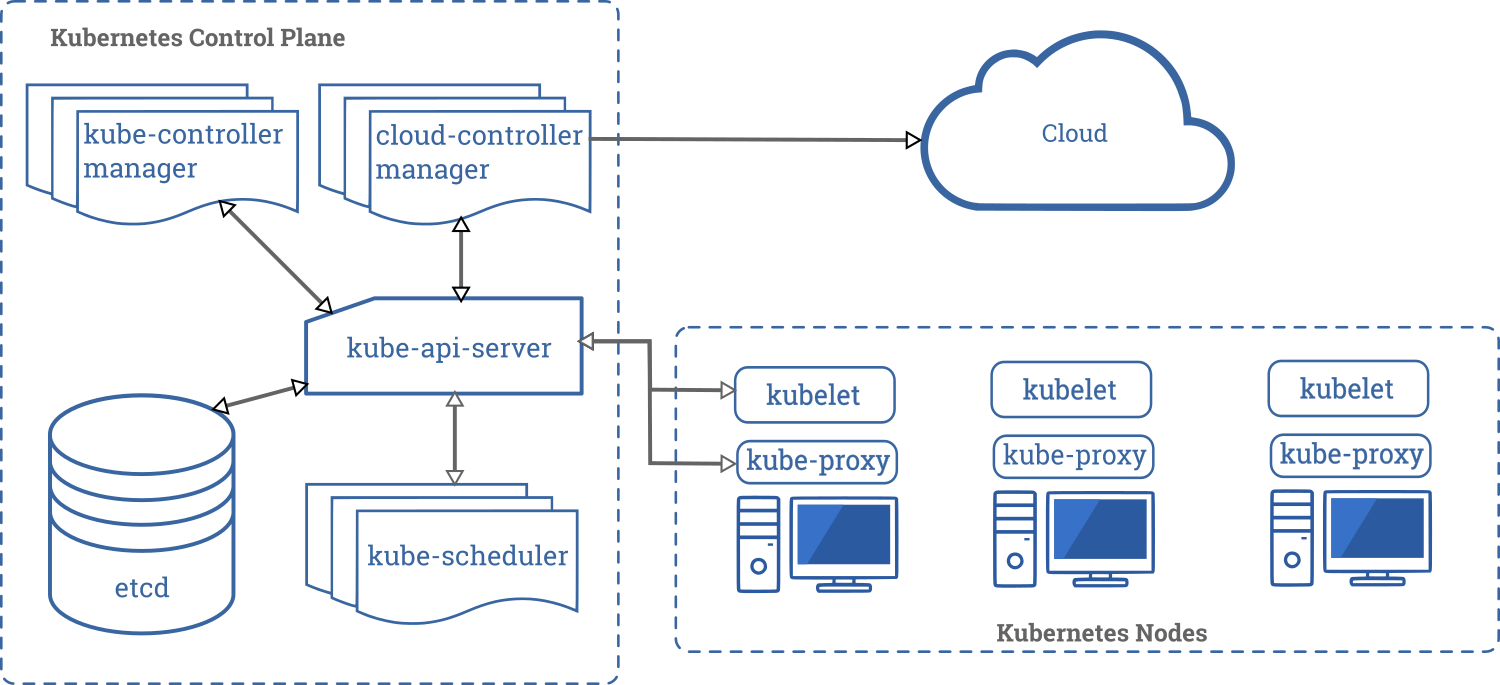
\includegraphics[width=1.0\textwidth]{./Figure/Kubernetes_Architettura.png}
 \caption{Architettura di Kubernetes}
 \label{fig:Architettura}
\end{figure}

\subsection{Componenti del Control Plane}
Il Kubernetes Control Plane è il centro nevralgico delle operazioni del cluster. È costituito da una serie di componenti, in esecuzione all'interno del cluster, che hanno il compito di garantire l'integritá esecutiva del cluster come ad esempio lo scheduling dei Worker Node e la gestione dei possibili errori dei Pod.
\begin{itemize}
    \item\textbf{kube-apiserver}
    è il server API per il cluster Kubernetes. È il punto di contatto centrale a cui accedono tutti gli utenti, l'automazione e i componenti nel cluster Kubernetes. Il server API implementa un'API RESTful su HTTP, esegue tutte le operazioni API ed è responsabile dell'archiviazione degli oggetti API in un backend di archiviazione persistente.
    \item\textbf{etcd}
    è la componente di archiviazione principale di Kubernetes, etcd memorizza e replica tutti gli stati dei cluster Kubernetes. Il meccanismo di memorizzazione che adotta è di tipo chiave-valore ovvero ad ogni valore memorizzato viene associato una chiave che rappresenta il suo identificatore univoco. In questo modo il Control Plane è in grado di storicizzare gli stati del Cluster confrontando lo stato attuale con quello desiderato in modo di intervenire tempestivamente in caso di necessità.
    \item\textbf{kube-scheduler}
    è la componente che consente al Control Plane lo scheduling dei Pod sui nodi. il kube-scheduler controlla i pod appena creati che non hanno un nodo assegnato, e dopo averlo identificato glielo assegna. 
\end{itemize}
\subsection{Componenti del Worker Node}
Il Worker Node è il nodo del cluster su cui viene eseguito effettivamente l'applicazione. Su ogni nodo di tipo Worker Node vengono eseguiti tre componenti di Kubernetes.
\begin{itemize}
    \item{kubelet}
    La componente kubelet è un agente che è sempre in esecuzione su ogni Worker Node e ha come compito quello di controllare il ciclo di vita dei container all'interno dei Pod. La kubelet riceve un set di specifiche definite in fase di deployment dall'utente e si assicura che i container rispettino tali specifiche.
    \item{kube-proxy}
    La componente kube-proxy è un proxy eseguito su ogni Nodo, ossia un particolare componente che consente di identificare i nodi all'interno della rete del cluster e permette che essi possano comunicare sia all'interno che all'esterno del cluster.
    \item{Container Runtime} il Container Runtime è il software responsabile dell'esecuzione dei container. Kubernetes supporta tutte le implementazioni di Kubernetes CRI (Container Runtime Interface) come ad esempio Docker e containerd.
\end{itemize}
\subsection{Oggetti Kubernetes}
Kubernetes offre una varietà di oggetti per definire le specifiche del proprio sistema. Questi oggetti costituiscono entità persistenti per rappresentare lo stato del cluster, quali applicazioni sono in esecuzione e su quali nodi, le risorse da allocare e le politiche da adottare. Per istanziare un oggetto con le direttive e le informazioni desiderate, si utilizza spesso un file di tipo YAML oppure JSON.
Ciascun oggetto è caratterizzato da due campi che ne descrivono la configurazione: \\\\
\textbf{Specifiche} Le specifiche descrivono lo stato desiderato dell'oggetto, cioè le caratteristiche che deve assumere. \\\\
\textbf{Stato} Lo stato descrive lo stato attuale dell'oggetto e viene automaticamente aggiornato da Kubernetes.
\begin{itemize}
    \item\textbf{Pod}
    Un Pod costituisce la più semplice, piccola e basilare unità di esecuzione in Kubernetes. La sua natura funzionale è quella di incapsulare uno o più container e di condividerne le risorse come l'archiviazione dei dati e le risorse di rete.
    I Pod generalmente non vengono creati direttamente in Kubernetes perchè questi sono considerati oggetti effimeri. Solitamente i Pod vengono creati e gestiti da controller di più alto livello come Deployment, StatefulSet o DaemonSet.
    \item\textbf{Deployment}
    L'oggetto Deployment si occupa di creare e gestire il ciclo di vita di uno o più Pod e dei ReplicaSet.
    Un Deployment fornisce un approccio dichiarativo per la creazione e la modifica di Pod e ReplicaSet, con esso è possibile dunque descrivere lo stato che il Pod deve assumere ed il Deployment Controller si occuperà di aggiornare lo stato attuale con quello desiderato.
    \item\textbf{ReplicaSet}
    Un ReplicaSet ha il compito specifico di mantenere attive una o più copie di un Pod. Questo meccanismo garantisce la piena disponibilità del Pod a cui il ReplicaSet è agganciato in quanto nel momento in cui un Pod, per un qualsiasi motivo, cessa il suo funzionamento, verrà sostituito da una sua esatta copia.
    \item\textbf{Service}
    I Pod in Kubernetes sono entità effimere, essi vengono creati e distrutti in base allo stato desiderato del cluster. Per natura quindi non hanno un'identificazione statica all'interno della rete del cluster ma ad ogni Pod viene assegnato un indirizzo IP dinamico che varia nel tempo.
    Un Service in Kubernetes costituisce un'astrazione che definisce un insieme logico di Pod e una politica con cui accedervi.
    Kubernetes offre diversi tipi di Service:
        \subitem\textbf{ClusterIP} Espone il Service con un indirizzo IP interno al cluster, rendendo il cluster raggiungibile solo dall'interno del cluster stesso.
        \subitem\textbf{NodePort} Espone il Service su ciascun indirizzo IP corrispondente ad un nodo del cluster, su una porta scelta automaticamente, uguale per tutti i nodi.
        \subitem\textbf{LoadBalancer} Permette di esporre le applicazioni all'esterno del cluster.
    \item\textbf{Job}
    Un oggetto di tipo Job permette di eseguire e gestire task complessi all'interno del cluster. Un Job infatti permette di eseguire un insieme di Pod in maniera sequenziale o parallela considerandoli come un'unica attività di lavoro da portare a termine. Il Job terrà in esecuzione l'attività fino a quando un numero specifico di Pod non verrà terminato correttamente. Quando viene raggiunto un numero specifico di completamenti riusciti, l'attività risulterà completata ed il Job cesserà la sua esecuzione. L'eliminazione del Job distruggerà dunque tutti i Pod precedentemente assegnati. 
\end{itemize}


% %%%%%%%%%%%%%%%%%%%%%%%%%%%%
\chapter{Stato dell'Arte}
La crescente popolarità dell’approccio multi-cloud ha portato alla nascita di varie tecnologie che ne permettano l’utilizzo, ognuna delle quali utilizza un approccio specifico in base agli obiettivi che si pone. Inizialmente lo scopo degli strumenti era quello di fornire un modo per unificare la gestione e il controllo delle varie risorse fornite dai diversi provider, raggruppandole sotto un unico ambiente. È il caso di OpenStack \cite{OpenStack}, un software open-source rilasciato sotto licenza Apache che opera come un sistema operativo per Cloud. OpenStack permette di creare e gestire ambienti Cloud, sia pubblici che privati, attraverso risorse virtuali relative al modello IaaS, di conseguenza manca il supporto agli altri modelli, soprattutto al Serverless Computing. Un approccio simile è seguito da MODAClouds \cite{MODAClouds}, un framework che segue un approccio model-driven per la progettazione e l’esecuzione di applicazioni multi-cloud. Il punto di forza è il suo approccio model-driven che consente di progettare le applicazioni ad alto livello, in completa astrazione rispetto al Cloud di riferimento, e poterle eseguire su qualsiasi piattaforma. Il codice in questione viene infatti tradotto in base all’ambiente di esecuzione permettendo una facile integrazione di più servizi Cloud e rendendo particolarmente semplice la migrazione delle applicazioni da provider a provider. \\
Con l’avvento del Serverless Computing è nata la necessità di estendere gli strumenti esistenti per supportare questo modello. È il caso di TOSCA \cite{TOSCASite}, acronimo per
Topology and Orchestration Specification for Cloud Applications, un linguaggio di standard OASIS per la modellazione per lo sviluppo e la gestione di applicazioni su Cloud. In \citet{TOSCAServerless} viene esteso per integrare la possibilità di sfruttare le componenti Serverless all’interno delle applicazioni che si vuole creare. TOSCA permette di descrivere la struttura e il comportamento dei servizi forniti dal Cloud concentrandosi su portabilità e interoperabilità delle applicazioni descritte, risultando tuttavia mancante di alcune funzionalità critiche per le applicazioni Cloud in quanto non permette di specificare i requisiti di risorse. Un approccio molto simile è quello di CAMEL \cite{CAMELSite}, un Multi-Domain-Specific Language per la gestione del ciclo di vita delle applicazioni. Acronimo di Cloud Application Modelling and Execution Language, CAMEL consente di modellare componenti per applicazioni o servizi sfruttando più ambienti Cloud. Anche in questo caso il linguaggio viene esteso in \citet{@ServerlessCamel} che introduce un’estensione che supporti le componenti Serverless. CAMEL è un multi-DSL, l’unione di diversi DSL per coprire tutti gli aspetti del ciclo di vita di un’applicazione, ed è basato sulla tecnologia Xtext di Eclipse.
Basato su CAMEL MELODIC \cite{MELODIC} è un middleware che permette di automatizzare ed ottimizzare lo sviluppo di applicazioni multi-cloud. Tutte le componenti di MELODIC non sono legate ad un particolare Cloud provider ma possono essere utilizzate per qualsiasi ambiente su Cloud. L'integrazione all'interno di MELODIC del supporto alle componenti Serverless è descritto in \citet{ServerlessMultiCloud}. \\
Un altro tipo di soluzioni è quello dedicato esclusivamente alle componenti Serverless, di cui l’esponente maggiore è certamente Serverless \cite{ServerlessSite}, un framework web open-source scritto in Node.js. Serverless è il primo framework sviluppato per la costruzione di applicazioni basate sui servizi di Serverless Computing offerte dai principali Cloud provider, sono infatti supportati AWS Lambda di AWS, Azure Function di Microsoft Azure, IBM Bluemix e Google Cloud Platform. Serverless fornisce una CLI, Command Line Interface, per sviluppare le varie applicazioni fornendo esempi, strutture pre-costruite per agevolare il lavoro dello sviluppatore. Supportando tutti i maggiori Cloud provider, la Serverless Framework CLI fornisce un’esperienza di sviluppo singola per diversi provider. Punto a favore è la possibilità di testare le proprio applicazioni in locale, senza necessità di interagire con il provider, evitando quindi di incorrere in costi di esecuzione. Al contrario il limite di Serverless è proprio la specificità di servizio, dedicato alla costruzione di applicazioni puramente Serverless. \\
Un approccio diverso è proposto in \citet{DistributedFaas} in cui viene descritta un’architettura basata su container che permette di progettare e costruire un sistema distribuito tra diversi Cloud provider sul modello FaaS. Questa può essere vista come un’integrazione dei classici sistemi di High Performance Computing, formati da cluster di computer, declinati sul modello FaaS. Quello che si ottiene sono meccanismi di auto-scaling sia per macchine virtuali che per container in un ambiente distribuito multi-cloud, in aggiunta ad un sistema di bilanciamento del carico che tiene conto dei diversi cluster FaaS coinvolti. 


% %%%%%%%%%%%%%%%%%%%%%%%%%%%%
\chapter{Fly Language}
Per sviluppare un'architettura multi-cloud non basta raggruppare i vari servizi dei diversi Cloud provider in un unico sistema ma bisogna avere un approccio specializzato e ben ragionato. 
Bisogna creare infatti un ambiente omogeneo, tale da sfruttare efficacemente le cooperazioni fra i diversi Cloud provider, cercando di non rendere troppo difficile la sua gestione.
La difficoltà di costruire un ambiente multi-cloud risiede nella mancanza di standard nei vari servizi a disposizione. Ognuno dei diversi cloud provider mette a disposizione API e strumenti specifici per l'accesso e l'utilizzo dei propri servizi, costringendo lo sviluppatore a conoscerli tutti per la costruzione di un'architettura multi-cloud.
È chiaro quindi che, anche se il multi-cloud comporta enormi vantaggi nel suo utilizzo,esso risulta particolarmente complesso da utilizzare e da sfruttare facendo nascere il bisogno di strumenti che facilitino lo sviluppo di applicazioni basate sul multi-cloud\\
La chiave di volta nell’utilizzo del multi-cloud è sicuramente l’astrazione, 
ovvero l'utilizzo di strumenti che sollevano l'utente dalla necessità di conoscere tutti i dettagli implementativi per la gestione dell'ambiente, 
permettendo così di ottenere i vantaggi del multi-cloud evitando di introdurre complessità aggiuntiva \cite{ForbesMultiCloud}. 
A questo scopo è nato \textbf{Fly}, un \textbf{Domain-Specific Language} per il Calcolo Scientifico sul multi-cloud, al fine di sviluppare con facilità applicazioni che utilizzino la complessità computazionale elargita da diversi Cloud provider, grazie al paradigma FaaS, garantendo alte prestazioni ed alta scalabilità. 
Il punto di forza di Fly risiede nella gestione dell'interazione con il Cloud la quale viene completamente astratta all’utente finale che 
non necessita di conoscere le specifiche API del provider che vuole utilizzare \cite{ISISLab}. \\
La novità in Fly risiede nel concetto di \textbf{funzione Fly}, ovvero un blocco di codice indipendente eseguibile concorrentemente, in linea con il modello FaaS, che usufruisce di funzioni Serverless. \\


Le caratteristiche principali di Fly sono:
\begin{itemize}
    \item Fly è \textit{efficace} perché permette di sfruttare la potenza computazionale di diversi Cloud provider in poche righe di codice, utilizzando le soluzioni più efficienti in base alle necessità;

    \item Fly è \textit{chiaro} perché è un linguaggio user-friendly, che rimuove diverse preoccupazioni alle quali il programmatore dovrebbe tener conto
    come il dover gestire e configurare diversi ambienti di esecuzione;
    
    \item Fly è \textit{efficiente} perché permette di scegliere i servizi migliori sia dal punto di vista delle funzionalità che del costo, inoltre riduce i tempi di sviluppo grazie all'astrazione.
\end{itemize}

In questo capitolo saranno descritti i dettagli del linguaggio Fly, descrivendo gli obiettivi per cui è stato sviluppato, la sua architettura e il suo funzionamento. Viene inoltre introdotto il concetto di Domain-Specific Language e Xtext, il framework utilizzato per lo sviluppo di Fly.

\section{Obiettivi}
Fly ha come obiettivo congiungere il Cloud Computing con l’High Performance Computing, fornendo un applicativo potente, semplice ed efficace per lo sviluppo di applicativi in grado di sfruttare il sistema multi-cloud al massimo delle sue potenzialità. \\
I principali obiettivi di Fly sono:

\begin{itemize}
    \item \textit{espressività} - possibilità di scrivere applicativi in maniera precisa,intuitiva e comprensibile;
    
    \item \textit{alta usabilità} - scrivere ed eseguire un applicativo Fly sono operazioni che devono essere semplici e completamente 
    astratte dai processi necessari all'interazione con il Cloud Provider, eliminando così la necessità di conoscere le API del Cloud provider;
    
    \item \textit{scalabilità} - I processi eseguiti in locale come quelli eseguiti in ambiente Cloud devono essere altamente scalabili.
\end{itemize}

Fly è stato realizzato per permettere agli esperti di un particolare campo che non hanno padronanza dei concetti articolati che riguardano i sistemi paralleli e distribuiti,
 di implementare i propri algoritmi sfruttando il parallelismo mediante architetture Serverless. Infatti, la sintassi di Fly è ispirata a linguaggi come Java, JavaScript, Python e R. 
 Linguaggi utilizzati spesso nel Calcolo Scientifico. Vengono forniti numerosi costrutti specifici per il dominio di interesse che vanno a formare un ricco linguaggio utilizzabile facilmente per interagire con i servizi su Cloud. \\
Fly supporta in modo implicito il paradigma di calcolo distribuito e parallelo insieme con la gestione della memoria fornendo inoltre un sistema di comunicazione di processi tramite appositi canali di comunicazione. Un programma Fly è infatti eseguibile sia su un'architettura multiprocessore sia su ambiente Cloud che supporti il modello FaaS, il tutto senza la necessità di conoscere in maniera precisa le risorse di computazione che occorrono per l'esecuzione \cite{ISISLab}.

Quando si parla di un \textbf{Domain-Specific Language (DSL)} si intende un linguaggio di programmazione sviluppato per l'utilizzo nel contesto di un particolare dominio, che elargisce una notazione su misura fondata sui criteri e sulle caratteristiche principali per tale dominio.
Mentre i linguaggi General Purpose possono essere utilizzati in molteplici situazioni e problemi, i DSL invece ne rappresentano il concetto opposto. Utilizzando un DSL si introduce un livello di astrazione tale da rendere possibile la realizzazione di soluzioni efficaci senza aver bisogno di competenze tecniche  specifiche anche ad esperti del dominio. Lo sviluppo di applicazioni software può così essere affidato a figure con conoscenze del contesto più specifiche e non più soltanto ai soli informatici, in modo da aumentare efficienza ed efficacia del procedimento.\\
Un DSL però non è genericamente utile a tutti, è invece ideato per la risoluzione di problemi riguardanti contesti molto specifici.
Fra i DSL possiamo prendere come esempio HTML, che è stato pensato per sviluppare siti web ma di certo non è compatibile, ad esempio, con la costruzione di applicazioni di simulazione, dominio a cui invece è dedicato OpenABL. Altri esempi di DSL potrebbero essere invece SQL per la stesura di query su database relazionali, che permette di scrivere interrogazioni semplici per l'ottenimento di dati senza la necessità delle competenze di un amministratore di database. \\
Il motivo per cui nasce un DSL è quello di essere di facile comprensione ed impiego, merito della forte specificità di utilizzo, divenendo così espressivo, piccolo e poco ridondante e permettendo a sviluppatori ed esperti del dominio di utilizzarlo come punto d'incontro. \\
Per la costruzione di un DSL è necessario realizzare un compilatore capace di leggere il programma scritto in quello specifico linguaggio, esaminarlo, processarlo e interpretarlo per poter infine generare il codice eseguibile. Andranno quindi attraversate una serie di fasi esposte a seguire:

\begin{itemize}
    \item \textit{analisi lessicale} - il programma iniziale viene suddiviso in singole unità chiamate \textit{token}, ognuna delle quali corrisponde ad un singolo elemento del linguaggio;
    
    \item \textit{analisi sintattica} - i \textit{token} identificati vengono analizzati per assicurarsi che formino uno statement valido per il linguaggio. È in questa fase che viene prodotto l’Abstract Syntax Tree (ABS), ovvero la rappresentazione della struttura sintattica del programma;
    
    \item \textit{analisi semantica} - comprende la fase di type checking che controlla che gli assegnamenti di valore siano compatibili con il relativo tipo di dati insieme con la fase di tracciamento degli identificatori, del loro tipo e delle espressioni che si assicura anche che i primi siano stati dichiarati prima dell’uso;
    
    \item \textit{generazione del codice} - parte finale che utilizza i risultati delle fasi precedenti per generare il codice macchina o, eventualmente, il programma scritto in un altro linguaggio.
\end{itemize}

\subsubsection{Xtext}
\textbf{Xtext} \cite{Xtext} è un framework open-source per lo sviluppo di linguaggi di programmazione e DSL. Diversamente dai comuni strumenti disponibili, Xtext genera non solo un parser ma anche un class model per l’Abstract Syntax Tree, fornendo anche un IDE, ovvero un ambiente di sviluppo, basato su Eclipse completo di tutte le funzioni e personalizzabile. Lo sviluppo di un linguaggio attraverso Xtext si basa sulla scrittura di una grammatica che lo definisce in tutte le sue parti, essa permette di ottenere un’infrastruttura completa inclusa di parser, linker, typechecker e compilatore insieme con il supporto all’editing per Eclipse. L’utilizzo di un framework come Xtext offre enormi vantaggi agli sviluppatori di DSL ed è per questo motivo che è stato scelto per la creazione del compilatore source-to-source di Fly.

\section{Architettura}
L'architettura di Fly è stata realizzata in modo tale che le risorse dell'applicativo sviluppato dall'utente vengano stabilite in maniera automatica in base ai requisiti computazionali.
Essa supporta due modelli di esecuzione: in locale ed in Cloud.
Quando si esegue l'applicativo Fly in locale, è la macchina ospitante a farsi carico dell'intero carico computazionale richiesto mentre se lo stesso applicativo viene eseguito in ambiente Cloud allora 
l'esecuzione del codice avviene attraverso un'architettura di calcolo parallelo grazie a costrutti specifici atti a facilitare l'esperienza dell'utente.
Fly risulta un linguaggio staticamente e fortemente tipizzato che sfrutta varie tipologie di inferenza per determinare il tipo delle variabili e delle costanti dichiarate.
Un programma scritto in Fly viene tradotto in automatico dal compilatore in codice Java, nello specifico ogni tipo di dato presente all'interno di Fly ha un suo corrispettivo in quest'ultimo linguaggio, 
così come le varie funzionalità specifiche del dominio vengono realizzate sfruttando l'ampia gamma di metodi offerti dal linguaggio General Purpose. \\
L’elemento fondamentale di Fly è rappresentato dal concetto di \textbf{funzione Fly}, ovvero una porzione di codice indipendente che eseguita in maniera concorrente, 
similmente a quanto avviene con le funzioni Serverless del modello FaaS. Le funzioni Fly possono essere eseguite in sequenziale o in parallelo, sia su infrastruttura locale multi-processore che su Cloud
 mediante l'utilizzo di appositi costrutti che ne permette la definizione, l'esecuzione, la sincronizzazione e la gestione della comunicazione. 
 Quest’ultima viene resa disponibile anche tra processi differenti in esecuzione su diversi ambienti attraverso l'uso di appositi canali di comunicazione virtuali i quali rappresentano 
 il metodo principale per lo scambio di dati tra diverse funzioni Fly. \\ 

\begin{figure}[htbp]
 \centering
 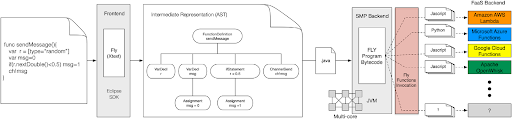
\includegraphics[scale=0.7]{./Figure/FLYCompilazione.png}
 \caption{Flusso di compilazione di Fly.}
 \label{fig:compilazione}
\end{figure}

La \figurename~\ref{fig:compilazione} mostra il \textbf{flusso di una compilazione} in Fly. Partendo da sinistra il programma Fly viene fornito in input al compilatore che genera un \textit{Abstract Syntax Tree (AST)}, ovvero un albero rappresentante la struttura sintattica del codice in cui ogni costrutto corrisponde ad un nodo. Viene definito astratto in quanto non vengono rappresentati tutti i dettagli del codice sorgente ma solo la sua struttura. In seguito la rappresentazione in AST intermedia viene trasformata in un programma Java da cui vengono estratte le singole funzioni Fly, ognuna delle quali verrà tradotta in diversi codici eseguibili, uno per ogni ambiente dichiarato dall’utente. Infine, osservando il lato destro della \figurename~\ref{fig:compilazione} è possibile osservare l’output finale che consiste nel codice compilato delle funzioni Fly pronto per essere eseguito sui vari ambienti dichiarati.

\begin{figure}[htbp]
 \centering
 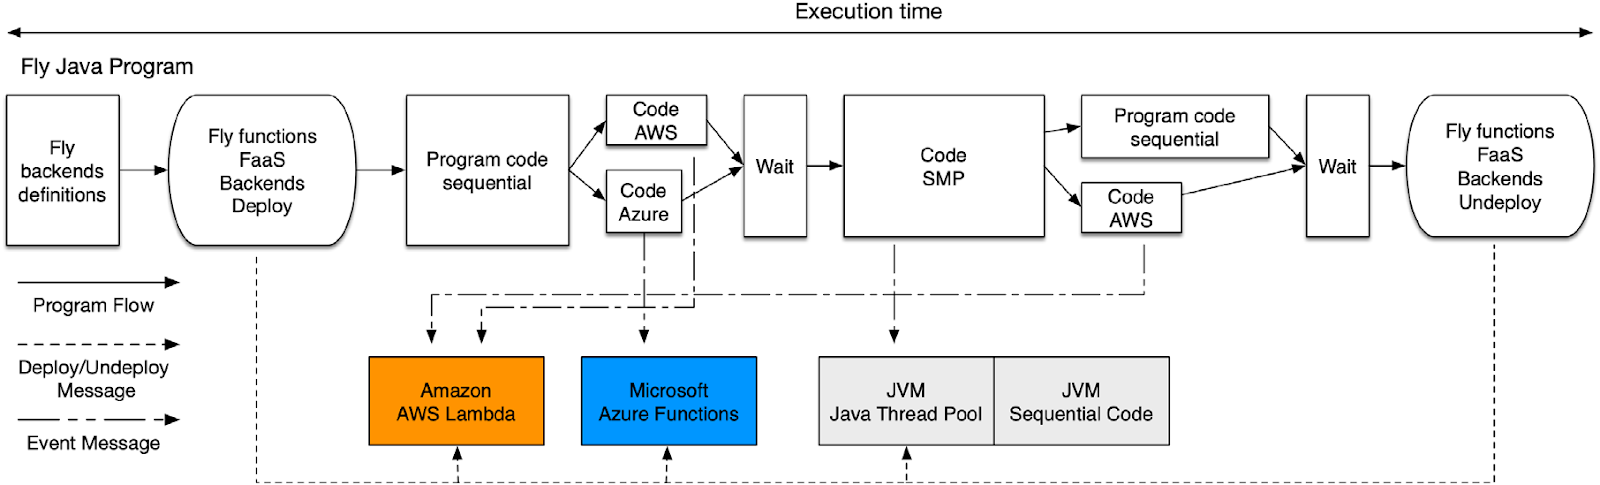
\includegraphics[scale=0.22]{./Figure/FLYEsecuzione.png}
 \caption{Flusso di esecuzione di Fly.}
 \label{fig:esecuzione}
\end{figure}

Nella \figurename~\ref{fig:esecuzione} viene mostrato nel dettaglio il flusso di esecuzione che inizia al lancio di un programma Fly. Seguendo il tempo di esecuzione, la prima fase prevede l’inizializzazione degli ambienti di back-end dichiarati all’interno del codice, questa prevede il login sul Cloud provider e l’istanziazione dei servizi necessari. Il codice generato a partire dalla funzione Fly viene poi caricato sul rispettivo ambiente Cloud, esso risulterà già compilato nel momento in cui il programma principale viene lanciato, in questo modo si evitano i tempi di attesa che sarebbero causati da una compilazione a tempo di esecuzione. Effettuata la fase di inizializzazione il programma principale viene mandato in esecuzione seguendo le istruzioni contenute nel codice Fly e al suo termine vengono effettuate una serie di procedure di undeploy sull’ambiente di back-end, avente lo scopo di eliminare tutte le istanze dei servizi Cloud creati in precedenza.

\section{Definizione del linguaggio}
Fly fornisce diversi tipi di dati che possono essere raggruppati in due insiemi, \textit{basici} e di \textit{dominio}. I primi sono ereditati da Java e comprendono \textit{booleani}, \textit{interi}, \textit{reali} e \textit{stringhe}, essi possono essere usati anche per la dichiarazione di array monodimensionali, bidimensionali e tridimensionali. Di numero maggiore sono invece i tipi di dominio utilizzabili in Fly che permettono all'utente di interagire e comunicare con l'ambiente di esecuzione.\\
Il Listato~\ref{lst:pigreco} mostra un semplice esempio di programma Fly per il calcolo di una stima di Pi Greco tramite il metodo Monte Carlo su ambiente Amazon Web Services, in particolare sfruttando il servizio AWS Lambda \cite{LambdaSite}. È utile fornire una prima descrizione del codice i cui elementi verranno poi approfonditi in seguito. Alla Riga 1 troviamo la dichiarazione dell'ambiente di esecuzione, in questo caso viene definito su AWS. Su tale ambiente è dichiarato un \verb|channel|, Riga 3, che permette al programma principale di comunicare con la funzione Fly \verb|hit| definita alla Riga 5, la quale genera un punto casuale e calcola se appartiene o meno ad un cerchio che abbia origine al punto 1.0, realizzando l'algoritmo per il metodo Monte Carlo. Il valore ottenuto viene poi inviata sul canale \verb|ch|. La funzione \verb|estimation|, Linea 16, legge l'output della funzione \verb|hit| e scrive a schermo la stima di Pi ottenuta. Alla linea 28 è possibile vedere come sono lanciate le funzioni Fly, in particolare viene utilizzata la parola chiave \verb|fly| per eseguire 10000 funzioni \verb|hit| sull'ambiente AWS. Infine l'utilizzo della parola chiave \verb|thenall| fa in modo che quando tutte le funzioni \verb|hit| hanno terminato venga eseguita la funzione \verb|estimation|.\\

\begin{lstlisting}[language=FLY,caption={Stima di PI Greco usando il metodo Monte Carlo su ambiente AWS.}, label={lst:pigreco}]
var local = [type="smp", nthread=4]

var cloud = [type="aws", user="user_name", access_id_key = "access_id_key", secret_access_key="secret_access_key", region="eu-west-2", language="nodejs12.x", thread=2, memory=256, time_=300]

var ch = [type="channel"] on cloud

func hit(){	
    var r = [type="random"]
    var x = r.nextDouble()
    var y = r.nextDouble()
    var msg = 0
    
    if((x * x)+(y * y) < 1.0){msg = 1}
    ch!msg on cloud
}


func estimation(){
    var sum = 0
    var crt = 0
    for i in [0:2] {
        sum += ch? as Integer
        crt += 1
    }
    println "pi estimation: " + (sum*4.0) \ crt
}

fly hit in [0:2] on cloud thenall estimation  
\end{lstlisting}  

\subsubsection{Object} 
Il principale tipo di dato di dominio è il tipo \verb|object|, un insieme eterogeneo di elementi di tipo basico e/o di dominio. Un Fly \verb|object| può essere visto come l'unione di un \verb|array|, un classico vettore, e di una \verb|mappa|, ovvero una struttura dati in grado di memorizzare elementi nella forma di coppie chiave-valore. Il valore di un elemento può essere ottenuto in due diversi modi, utilizzando la sua posizione, come si fa per gli array, o la sua chiave, come nel caso di una mappa. Quando un nuovo valore è assegnato ad una data chiave o posizione viene creato un nuove elemento, altrimenti il nuovo valore va a sostituire il precedente. \\
Ogni tipo di dato di dominio presente in Fly è un'istanza del tipo \verb|object|, questo fa sì che essi siano costruiti tutti con una sintassi simile utilizzando il campo \verb|type| per specificarne il tipo.

\subsubsection{Ambiente di esecuzione}
Il codice di un programma Fly inizia sempre con la dichiarazione di uno o più \textbf{ambienti di esecuzione}, necessari affinché il generatore possa configurare le risorse utili al funzionamento dell'applicazione, in particolare è sempre necessario un ambiente di esecuzione locale corrispondente alla macchina su cui viene lanciato il programma. Ad esempio nel caso di un ambiente locale multiprocessore viene utilizzata una \verb|Java Thread Pool| mentre per gli ambienti su Cloud è necessario creare le istanze dei servizi necessari. Il grande vantaggio offerto da Fly è l'astrazione, dal punto di vista dello sviluppatore infatti tutti i tipi di ambienti possono essere utilizzati allo stesso modo, sarà il compilatore ad occuparsi dei dettagli implementativi specifici relativi al loro utilizzo. \\
La dichiarazione di un ambiente di esecuzione necessita di una serie di parametri che variano in base alla tipologia di ambiente, specificata dal campo \verb|type|. Oltre ad eventuali informazioni aggiuntive richieste dai diversi Cloud provider per accedere ai loro servizi, la dichiarazione relativa ad un'esecuzione su Cloud richiede che l'utente specifichi il linguaggio di programmazione in cui verranno tradotte le funzioni Fly per essere lanciate sul servizio Serverless del provider. In particolare le possibilità sono JavaScript \cite{JavaScriptSite} o Python \cite{PythonSite}.\\
Attualmente gli ambienti supportati sono tre:

\begin{itemize}
    \item \textbf{smp} - ambiente locale che sfrutta il parallelismo basato su un sistema multiprocessore simmetrico sfruttando i thread Java;
    
    \item \textbf{aws} - ambiente su Cloud legato al provider Amazon Web Services (AWS)  \cite{AmazonSite} che sfrutta il servizio AWS Lambda \cite{LambdaSite} per eseguire le funzioni Fly;
    
    \item \textbf{azure} - ambiente su Cloud legato al provider Microsoft Azure \cite{MicrosoftSite} che sfrutta il servizio Azure Function \cite{FunctionSite} per eseguire le funzioni Fly. In questo caso il supporto a Python non è previsto in quanto al momento dell'implementazione non ancora reso disponibile da Azure.
\end{itemize}

\subsubsection{Channel}
La comunicazione e la sincronizzazione sia tra le varie funzioni Fly, sia tra queste e il programma principale avviene mediante la dichiarazione di un \verb|type|\verb|=|\verb|"channel"| che necessita di specificare l'ambiente di esecuzione sul quale funzionare mediante la parola chiave \verb|on|. Questo metodo di comunicazione segue il modello delle code di messaggi bloccanti, ovvero quando si tenta di ricevere un messaggio l'esecuzione si ferma fino a che un nuovo messaggio non viene ricevuto. L'utilizzo del carattere \verb|"!"| permette l'invio di messaggi, vedi Riga 13 del Listato~\ref{lst:pigreco}, mentre il carattere \verb|"?"| è necessario per la loro ricezione, vedi Riga 22 del Listato~\ref{lst:pigreco}. Fly implementa un meccanismo di serializzazione in quando la comunicazione utilizza le infrastrutture di rete per scambiare messaggi con l'ambiente su Cloud.

\subsubsection{Funzione Fly}
Le \textbf{funzioni Fly} sono già state in parte descritte, esse sono frammenti di codice scritto per realizzare una funzionalità specifica indipendente dal programma principale e da altre funzioni ed eseguibile in maniera concorrente. Queste funzioni sono ben diverse da quelle disponibili in altri linguaggi di programmazione e prendono ispirazione da quelle utilizzate nei linguaggi funzionali.\\
La dichiarazione di una funzione Fly è possibile utilizzando la parola chiave \verb|func| a seguito della quale si definisce il nome della funzione e si inseriscono eventuali parametri di input tra parentesi che vengono passati per copia e sono considerati immutabili. Le funzioni Fly possono restituire un valore mediante l'uso della parola chiave \verb|return| ed hanno scoping privato, ovvero solo i parametri della funzione e le variabili locali sono visibili all'interno del corpo della funzione. Per superare tale limitazione possono essere utilizzati sia gli oggetti \verb|channel| che le costanti a patto che la dichiarazione e l'accesso avvengano nello stesso ambiente di esecuzione. Questo significa che se una funzione è in esecuzione sull'ambiente X essa può utilizzare canali e oggetti disponibili su tale ambiente X a prescindere da chi li abbia dichiarati.
Le funzioni Fly possono essere eseguite in modo concorrente utilizzando la parola chiave \verb|fly|, non essendo ammessa la ricorsione essa non può essere utilizzata all'interno del corpo di una funzione. Il suo utilizzo causa la generazione di un evento sull’ambiente che si sta utilizzando, sia esso SMP o su Cloud, in modo che le funzioni vengano eseguite, in linea con il modello di programmazione event-driven che caratterizza il Serverless Computing. Il parallelismo esplicito da cui è caratterizzato Fly è racchiuso nel modo in cui vengono lanciate le funzioni, a seguito della parola chiave \verb|fly| viene dichiarata il nome della funzione da eseguire e, se necessario, il loro numero insieme alla variabile che rappresenta l'ambiente di esecuzione da utilizzare specificato in seguito alla parola chiave \verb|on|.

\subsubsection{Funzione di Callback}
Le \textbf{funzioni di Callback} sono funzioni Fly che vengono eseguite al termine dell'esecuzione di una precedente funzione. Esse possono essere dichiarate dopo la specifica dell'ambiente di esecuzione su cui deve essere eseguita una funzione Fly. Due tipi di funzioni di Callback sono supportate, la prima riguarda quelle specificate in seguito alla parola chiave \verb|then| che indica che la sua esecuzione deve avvenire dopo ogni singola funzione Fly, mentre utilizzando la parola chiave \verb|thenall| si richiede che la funzione venga eseguita solamente quando tutte le funzioni Fly hanno terminato.

\subsubsection{Esecuzioni asincrone}
Fly permette \textbf{esecuzioni asincrone} attraverso l'uso della parola chiave \verb|async| e tipo di dato di dominio chiamato \verb|async-object| che permette all'utente di controllare ed interagire esse. Invocando una funzione utilizzando \verb|async| viene restituito immediatamente il controllo al programma principale in modo che l'esecuzione possa continuare, a questo punto l'utente può controllare lo stato delle funzioni asincrone usando il metodo \verb|status()| dell'\verb|async-object|, mentre il metodo \verb|wait()| mette in pausa l'esecuzione fino a che tutte le funzioni non hanno terminato.

\subsubsection{Codice nativo}
La possibilità di includere \textbf{codice nativo} all'interno di applicazioni Fly è data dalla parola chiave \verb|native|, tale funzionalità consente, ad esempio, di inserire in una funzione Fly codice scritto direttamente in Python ed esso non verrà tradotto o modificato dal compilatore Fly ma copiato così com'è. Tramite la parola chiave \verb|require| è inoltre consentito includere ed installare librerie esterne addizionali nell'ambiente di esecuzione.

\subsection{Struttura di un progetto Fly}
Fly utilizza il gestore di pacchetti \textit{Maven} \cite{MavenSite} per la costruzione e la generazione dei progetti. Maven è uno strumento per la gestione di progetti software e di build automation basato sul concetto di \textbf{Project Object Model (POM)}, un file XML che contiene le dipendenze necessarie al funzionamento dell'applicazione. \\
La creazione di un \textbf{progetto Fly} genera due cartelle principali insieme con un file POM, il tutto racchiuso in un progetto Java Maven che include tutte le dipendenze, il programma principale e il codice delle funzioni, il tutto costruito sulla base del programma Fly da parte del compilatore. Attraverso il comando \verb|mvn package| di Maven tale progetto viene utilizzato per la generazione del file \textit{JAR} eseguibile \cite{ISISLab}.\\
Un progetto Fly è così strutturato:

\begin{itemize}
    \item \textbf{cartella \textit{src}} - cartella in cui è posizionato il file con estensione \textit{.fly} contenente il codice del programma scritto in linguaggio Fly;
    
    \item \textbf{cartella \textit{src-gen}} - cartella contenente i file generati dal compilatore che consistono in un file Java e due file di script. Il file Java ha il compito di orchestrare l'intera esecuzione del programma, ovvero l'intero ciclo di vita comprensivo del lancio dei due file di script. Questi ultimi sono file con estensione \textit{.sh} e contengono distintamente i comandi per il deploy delle funzioni Fly e le procedure per l'undeploy. Il file di deploy si occupa di creare il file necessario alla creazione della funzione Serverless sul servizio FaaS del provider definito, comprensivo di codice, librerie e file di configurazione, mentre il file di undeploy ha il compito di ripulire l'ambiente Cloud dalle risorse create;
    
    \item \textbf{file XML \textit{pom.xml}} - unità fondamentale di Maven per la gestione del progetto, si tratta di un file XML che contiene informazioni e i dettagli di configurazione necessari per effettuare la build, nel caso specifico al suo interno sono presenti le librerie necessarie al programma \cite{MavenPom}.
\end{itemize}

\section{Generazione del codice}
Il punto di forza di Fly è quello di fornire un livello di astrazione tale per cui l'utente non deve conoscere le API di ogni Cloud provider per scrivere un programma che sfrutti al meglio i suoi servizi. Tali API restano comunque essenziali per interagire con essi, infatti è il compilatore di Fly che si occupa di prendere in input il programma per tradurlo in codice effettivamente eseguibile. È quello che avviene nella fase di generazione del codice in cui ogni componente scritta in linguaggio Fly viene trasformata nel linguaggio di destinazione, il quale varia a seconda del contesto, come visto nei paragrafi precedenti. Possiamo quindi affermare che il fulcro del compilatore di Fly è sicuramente la parte di generazione di codice che produce un programma diverso in base all’ambiente di esecuzione dichiarato dall’utente. Nel caso di un ambiente multiprocessore il parallelismo viene implementato attraverso l’uso di una \verb|Java Thread Pool| che permette l'utilizzo di thread ai quali viene assegnata una specifica esecuzione, in particolare essa permette di riutilizzare thread precedentemente creati, eliminando il tempo necessario alla loro creazione. Il programma Fly viene quindi eseguito su una \textit{Java Virtual Machine (JVM)} come un classico programma Java, sulla quale viene eseguito anche l’ambiente SMP, assumendo quindi che siano disponibili almeno due core fisici, uno per l’esecuzione del programma e uno per l’ambiente. L'esecuzione su Cloud prevede invece l'utilizzo delle API fornite dal provider di riferimento che consentono di interagire con i servizi disponibili in base ai quali vengono tradotti i vari costrutti e funzionalità di Fly.\\
Il codice generato per le funzioni Fly varia in base all'ambiente di esecuzione scelto, in particolare il linguaggio di destinazione può essere Java, JavaScript o Python in base a quanto specificato dall'utente. In caso di esecuzione su ambiente SMP locale le funzioni sono tradotte in Java, in quanto eseguite su JVM, diversamente dal Cloud i cui servizi FaaS permettono solitamente l'esecuzione di codice in JavaScript o Python. Oltre al linguaggio utilizzato, l’ambiente di destinazione determina anche il modo in cui viene generato lo script di deploy che costruisce il pacchetto di esecuzione contenente codice sorgente e librerie. \\
Durante la fase di esecuzione l'interazione con il Cloud avviene mediante l'utilizzo degli strumenti di \textbf{Command Line Interface} forniti dai vari provider come la \textit{AWS CLI} \cite{awsCLI} o la \textit{Azure CLI} \cite{azureCLI}, mentre le funzioni vengono invocate con delle chiamate \textit{HTTP POST} asincrone, le quali assicurano la minor latenza permettendo al programma di continuare la sua esecuzione in attesa di risposta da parte del servizio.

\subsubsection{Amazon Web Services}
Amazon Web Services mette a disposizione diverse SDK che permettono di interagire con i suoi servizi praticamente con tutti i principali linguaggi di programmazione \cite{awsSDK}. Il programma principale, essendo scritto in Java fa uso delle \textit{AWS SDK for Java} \cite{AwsJavaSDK} che consentono di accedere a tutti i servizi forniti da AWS mediante delle API dedicate. Gli script di deploy e undeploy invece utilizzano la AWS CLI \cite{awsCLI} per creare le istanze di servizi necessarie al funzionamento del programma e per caricare le funzioni Fly e i relativi pacchetti su AWS Lambda. Queste ultime sfruttano la libreria \textit{boto3} per Python \cite{AwsPySDK} e la libreria \textit{aws-sdk} per JavaScript \cite{AwsJsSDK} per interagire con i servizi di AWS.

\subsubsection{Microsoft Azure}
Le SDK di Microsoft Azure soffrono di alcune problematiche di utilizzo derivanti sia dalla difficile integrazione al di fuori dell’IDE VisualStudio Code, sia dalla mancanza di funzionalità per gran parte dei servizi. Per questo motivo il supporto ad Azure passa per l’utilizzo di un servizio REST API che prescinde dal linguaggio di programmazione in quanto basato su operazioni HTML. Le \textit{Representational State Transfer (REST) API} consistono in endpoint specifici per ogni servizio che supportano un insieme di operazioni HTTP i quali forniscono l’accesso alle principali funzionalità di un servizio come la creazione, l’aggiornamento, la cancellazione o l’ottenimento di informazioni. L’utilizzo delle REST API è regolato dall’utilizzo di un token di autorizzazione ottenibile tramite il servizio Azure Active Directory che ne permette l’acquisizione fornendo i propri dati di accesso, in particolare ID, password e TenantID.
\newpage 
Le sezione seguenti analizzano come il codice scritto in Fly viene tradotto dal compilatore nei vari linguaggi di destinazione per generare i file eseguibili. Tutti i Listati mostrati fanno riferimento al programma  per il calcolo di Pi Greco, proposto nella sua interezza nel Listato~\ref{lst:pigreco}.

\subsection{Ambiente di esecuzione}

\subsubsection{Ambiente locale - SMP}
La dichiarazione di un \textbf{ambiente locale} necessita di due parametri, il primo definisce il tipo di ambiente che sarà di \verb|type|\verb|=|\verb|"smp"|, il secondo specifica il numero di thread che dovranno essere utilizzati.\\

\begin{lstlisting}[language=FLY,caption={Dichiarazione di un ambiente di esecuzione locale.}, label={lst:smp}]
var local = [type = "smp", nthread = 4]
\end{lstlisting}

Il codice Java generato risulta in un oggetto \verb|ExecutorService| che semplifica l'esecuzione asincrona, permettendo di eseguire i task in modo concorrente. Esso fornisce automaticamente un insieme di thread con una serie di metodi che permettono di assegnare loro dei task.\\

\begin{lstlisting}[language=Java,caption={Codice generato per l'ambiente di esecuzione locale.}, label={lst:localJava}]
static ExecutorService __thread_pool_local = Executors.newFixedThreadPool(4);
\end{lstlisting}

\subsubsection{Ambiente su Cloud - Amazon Web Services}
L'utilizzo di un ambiente di esecuzione che utilizzi il \textbf{Cloud AWS} è possibile mediante la dichiarazione di una variabile di \verb|type|\verb|=|\verb|"aws"| la quale necessita di una serie di parametri corrispondenti alle caratteristiche necessarie al lancio delle funzioni Serverless su AWS Lambda \cite{LambdaConfiguration}:

\begin{itemize}
    \item \textbf{dati di accesso dell'account AWS}: in ordine sono necessari \verb|user_name|, \verb| access_id_key|, \verb|secret_access_key|;
    \item \textbf{regione}: id della regione su cui si vogliono lanciare i servizi;
    \item \textbf{linguaggio}: linguaggio di programmazione in cui verranno tradotte ed eseguite le funzioni Lambda. Può essere \verb|nodejs| per JavaScript o \verb|python| per Python;
    \item \textbf{thread}: numero di istanze concorrenti da lanciare per l'esecuzione delle funzioni;
    \item \textbf{memoria}: quantità di memoria disponibile per l'esecuzione di una funzione;
    \item \textbf{time}: tempo limite di esecuzione per ogni funzione.
\end{itemize}



\begin{lstlisting}[language=FLY,caption={Dichiarazione di un ambiente Cloud su AWS.}, label={lst:aws}]
var cloud = [type="aws", user="user_name", access_id_key = "access_id_key", secret_access_key="secret_access_key", region="eu-west-2", language="nodejs12.x", thread=2, memory=256, time_=300]
\end{lstlisting}

Nel Listato~\ref{lst:awsJava} vediamo come vengono istanziati i servizi necessari all'esecuzione di un programma Fly utilizzando le informazioni fornite nella dichiarazione dell'ambiente. Tra i servizi troviamo AWS SQS \cite{SQS} per le code di messaggi, AWS IAM \cite{IAM} per l'autenticazione, AWS S3 \cite{S3} per la memorizzazione di dati e AWS Lambda \cite{LambdaSite} per l'esecuzione di funzioni Serverless.\\

\begin{lstlisting}[language=Java,caption={Codice generato per l'ambiente Cloud su AWS.}, label={lst:awsJava}]
static BasicAWSCredentials cloud = new BasicAWSCredentials("access_id_key", "secret_access_key");
		
static AmazonSQS __sqs_cloud  = AmazonSQSClient.builder()
	.withCredentials(new AWSStaticCredentialsProvider(cloud))
	.withRegion("eu-west-2")
	.build();
		
static AmazonIdentityManagement __iam_cloud = AmazonIdentityManagementClientBuilder.standard()
	.withCredentials(new AWSStaticCredentialsProvider(cloud))
	.withRegion("eu-west-2")
	.build();
			
static AWSLambda __lambda_cloud = AWSLambdaClientBuilder.standard()
	.withCredentials(new AWSStaticCredentialsProvider(cloud))
	.withRegion("eu-west-2")
	.build();
			
static AmazonS3 __s3_cloud = AmazonS3Client.builder()
    .withCredentials(new AWSStaticCredentialsProvider(cloud))
    .withRegion("eu-west-2")
    .build();
\end{lstlisting}

\subsubsection{Ambiente su Cloud - Microsoft Azure}
Utilizzare i servizi a disposizione sul \textbf{Cloud di Microsoft Azure} mediante linguaggi di programmazione risulta complesso e macchinoso a causa delle SDK fornite che, attualmente, presentano molteplici mancanze oltre ad una documentazione particolarmente scarna e spesso non aggiornata. Per tale motivo si è scelto di utilizzare il sistema di REST API attraverso delle chiamate \textit{HTTP}. L'integrazione dei servizi di Microsoft Azure all'interno del codice Java generato dal compilatore Fly è resa possibile grazie alla libreria AzureClient sviluppata presso l'ISISLab \cite{Grieco}, la quale permette di superare  della frammentazione delle SDK fornendo un'unica interfaccia che permette un più agevole utilizzo dei servizi. La gestione dei servizi di Azure con JavaScript soffre dei medesimi problemi in termini di SDK ed anche in questo caso è necessario utilizzare delle chiamate \textit{HTTP} per utilizzarli, in particolare vengono utilizzate le librerie \textit{axios} \cite{axios} e \textit{qs} \cite{qs}. In entrambi i casi rimane indispensabile il servizio Azure AD \cite{azureAD} per ottenere il \textit{token} di autorizzazione che permette di effettuare tali chiamate.\\
L'utilizzo di un ambiente di esecuzione che utilizzi il \textbf{Cloud Azure} è possibile mediante la dichiarazione di una variabile di \verb|type|\verb|=|\verb|"azure"| la quale necessita di una serie di parametri corrispondenti alle caratteristiche necessarie al lancio delle funzioni Serverless sul servizio Azure Function \cite{azureFunction}:il problema

\begin{itemize}
    \item \textbf{dati di accesso dell'account Azure}: in ordine sono necessari \verb|client_id|,  \verb|tenant_id|, \verb|secret_key|, \verb|subscription_id|;
    \item \textbf{regione}: id della regione su cui si vogliono lanciare i servizi;
    \item \textbf{linguaggio}: linguaggio di programmazione in cui verranno tradotte ed eseguite le funzioni Lambda. Può essere \verb|nodejs| per JavaScript o \verb|python| per Python;
    \item \textbf{thread}: numero di istanze concorrenti da lanciare per l'esecuzione delle funzioni;
    \item \textbf{time}: tempo limite di esecuzione per ogni funzione.
\end{itemize}



\begin{lstlisting}[language=Java,caption={Dichiarazione di un ambiente Cloud su Azure.}, label={lst:azure}]
var cloud = [type="azure", clientID="client_id", tenantID="tenant_id", secret_key="secret_key", subscriptionID="subscription_id", region="France Central", language="nodejs12.x", threads="2", seconds="300"]
\end{lstlisting}

Il codice generato, visibile nel Listato~\ref{lst:azureJava}, comprende la creazione di una variabile istanza della libreria AzureClient necessaria per avviare tutte le procedure relative ai servizi di Azure. In particolare il metodo \verb|init()| si occupa di istanziare tutti i servizi di base indispensabili per l'esecuzione di qualsiasi programma Fly, sfruttando le informazioni fornite nella dichiarazione dell'ambiente per effettuare l'accesso al Cloud. Il metodo \verb|createFunctionApp(...)| invece è adibito alla creazione dell'istanza del servizio Serverless di Azure che permette l'esecuzione delle funzioni.\\

\begin{lstlisting}[language=Java,caption={Codice generato per l'ambiente Cloud su Azure.}, label={lst:azureJava}]
cloud = new AzureClient("client_id",
    "tenant_id",
    "secret_key",
    "subscription_id",
    __id_execution+"",
    "France Central");
    
cloud.init();

cloud.createFunctionApp("flyappcloud","nodejs12.x");
\end{lstlisting}

\subsection{\textit{Channel}}
La dichiarazione di un \verb|type|\verb|=|\verb|"channel"|, ovvero il mezzo di comunicazione e sincronizzazione utilizzato da Fly, necessita come unica specifica l'ambiente di esecuzione su cui dovrà funzionare, come mostrato nel Listato~\ref{lst:flyChannel}. Questo viene specificato mediante la parola chiave \verb|on| e in base ad esso il compilatore genererà un codice differente, adattandolo in modo che sfrutti i servizi di gestione delle code forniti dall'ambiente specificato. In particolare per AWS si utilizza il servizio AWS Simple Queue Service (SQS) \cite{SQS} mentre per Azure si sfruttano i metodi presenti all'interno della libreria AzureClient.\\
La logica di funzionamento dei prevede che ad uno dei thread dell'ambiente locale venga associato il task di lettura della coda rimanendo costantemente in ascolto e non appena vengono intercettati dei messaggi essi vengono immediatamente scritti sul canale sul quale è possibile leggerli.\\

\begin{lstlisting}[language=Java,caption={Dichiarazione di un \textit{Channel} su Cloud.}, label={lst:flyChannel}]
var ch = [type="channel"] on cloud
\end{lstlisting}

\subsection{Script di deploy e undeploy delle funzioni}
Il funzionamento delle funzioni Serverless su un ambiente Cloud richiede una serie di procedure sia per il deploy che per l'undeploy che vengono eseguite mediante gli strumenti di Command Line Interface forniti dai provider, di conseguenza i comandi cambiano in base al Cloud ma al linguaggio utilizzato. Nonostante ciò queste procedure non sono particolarmente diverse tra loro in quanto tutti necessitano, oltre che del codice della funzione, di una serie di file in formato JSON sia per la specifica del ruolo e delle autorizzazione con le quali la funzione viene eseguita sia per indicare le dipendenze del codice. Fly costruisce l'intero pacchetto per l'esecuzione delle funzioni Serverless prima che queste vengano caricate su Cloud, in particolare questo contiene solo i vari documenti JSON ma anche le librerie necessarie per l'esecuzione che vengono installate mediante il gestore di pacchetti \textit{npm} \cite{npm} per JavaScript e \textit{pip} \cite{pip} per Python.\\
Il codice contenuto all'interno degli script può essere suddiviso in sezioni, ognuna delle quali si occupa di una fase necessaria per il funzionamento del programma, descritte di seguito.

\begin{itemize}
    \item\textbf{Verifica dei parametri e dei requisiti} La prima parte dello script si occupa di verificare che siano presenti i parametri necessari all'interazione con l'ambiente di esecuzione per poi salvarli in apposite variabili. Vengono poi effettuati una serie di controlli per assicurarsi che tutte i pacchetti necessari siano installati sulla macchina, come ad esempio le Command Line Interface.
    \item\textbf{Inizializzazione dei servizi} Attraverso la CLI viene inizializzato l'ambiente del provider di riferimento utilizzando i dati di accesso forniti nella dichiarazione dell'ambiente. In particolare per AWS è necessario creare un'istanza del servizio IAM \cite{IAM} mentre per Azure si effettua semplicemente il login.
    \item\textbf{Creazione del virtual env - Python} In caso il linguaggio scelto per la funzione sia Python è necessario creare un \textit{virtual env}, ossia di un ambiente virtuale isolato che l'interprete di Python utilizza per l'installazione di librerie e script.
    \item\textbf{Creazione del progetto locale} Mediante l'uso dei comandi \textit{bash} lo script crea il progetto Fly occupandosi sia della creazione delle cartelle che dei file. È in questa fase che vengono creati i file JSON necessari per configurare il servizio FaaS, contenenti parametri come il tipo di trigger da utilizzare, nel nostro caso HTTP, i permessi e le autorizzazioni.
    \item\textbf{Codice della funzione Fly Serverless} La funzione Fly viene tradotta nel codice scelto, JavaScript o Python, scritto all'interno di un file che viene inserito all'interno del progetto.
    \item\textbf{Deploy della funzione} Le procedure di deploy della funzione cambiano in base al all'ambiente scelto. AWS richiede che le librerie necessarie all'esecuzione siano già presenti all'interno del pacchetto che verrà caricato su Cloud, per questo motivo lo script utilizza i gestori di pacchetti \textit{npm} o \textit{pip} per la loro installazione per poi creare un file \textit{.zip} contenente l'intero progetto che viene usato per il deploy. A causa dei limiti di dimensione che tale pacchetto deve avere viene fatto un controllo aggiuntivo e in caso di superamento si utilizza il servizio di archiviazione S3 \cite{S3}. Il deploy per Azure risulta invece meno macchinoso in quanto le librerie necessarie vengono specificate all'interno di un file di requisiti che permette di mantenere la dimensione del progetto sempre molto contenuta.
    \item\textbf{Undeploy della funzione} Una volta eseguite le varie funzioni Fly lo script di undeploy si occupa di eliminare tutte le istanze dei servizi creati in modo da lasciare l'ambiente Cloud pulito. Questa fase viene effettuata tramite CLI per AWS mentre per Azure si utilizza la libreria AzureClient, di conseguenza lo script di undeploy contiene solo i comandi per effettuare il logout.
\end{itemize}

\subsection{Sincronizzazione}
L'esecuzione delle funzioni Fly su Cloud necessita di un sistema di sincronizzazione in grado di accertarsi che tutte le funzioni Fly abbiano terminato la loro esecuzione. Questo meccanismo viene implementato attraverso una coda di terminazione sulla quale ogni funzione invia un messaggio una volta completata. Mediante l'uso di un contatore il sistema può notificare che tutte le funzioni sono terminate nel momento in cui sono ricevuti tanti messaggi quante sono le funzioni lanciate. La coda di terminazione viene implementata con la stessa logica vista per i \verb|channel| in maniera totalmente astratta all'utente, essa viene creata, gestita ed eliminata dal programma stesso.


% %%%%%%%%%%%%%%%%%%%%%%%%%%%%
\chapter{Ambiente di esecuzione Kubernetes} \label{Kubernetes}
\section{Kubernetes in Fly}
Fly permette all'utente di sviluppare ed eseguire i propri applicativi senza preoccuparsi della gestione delle risorse, dell'ambiente su cui viene eseguito e tutto ciò che riguarda il ciclo di vita dell'applicativo stesso.
Ciò è possibile grazie al paradigma FaaS (Function as a Service), il quale permette di sfruttare i servizi offerti dai vari cloud provider per eseguire applicativi in ambienti serverless. Sebbene ciò abbia portato innumerevoli vantaggi nell'esecuzione e nella gestione del costrutto Fly, si riscontrano comunque delle problematiche e delle limitazioni:
\begin{itemize}
    \item gli ambienti serverless offerti dai diversi cloud provider limitano il tempo di esecuzione degli applicativi;
    \item le risorse disponibili per l'esecuzione del codice sono predefinite;
    \item l'ambiente in cui viene eseguito l'applicativo Fly è gestito dal Cloud Provider stesso. Un livello di astrazione così alto comporta l'impossibilità di gestire possibili errori e avere il pieno controllo dell'ambiente di esecuzione.
\end{itemize}

L'introduzione di un ambiente di esecuzione basato su Kubernetes all'interno di Fly permette di risolvere alcune di queste problematiche permettendo l'esecuzione delle funzioni Fly all'interno di un cluster Kubernetes. Ciò permette di avere un flusso di esecuzione simile a quello eseguito su ambiente serverless garantendo però un maggior controllo e meno limitazioni. La tecnologia sfruttata dai servizi di serverless computing, infatti, è basata sul lancio di container, ognuno dei quali si occupa dell'esecuzione di una singola funzione.
\section{Integrazione in Fly}
L'integrazione all'interno del linguaggio Fly, è stata progettata in modo da seguire le medesime sintassi e semantiche utilizzate per gli altri ambienti di esecuzione. Nello specifico, è stata introdotta l'entità \verb|K8s| la quale richiede tre campi necessari come si può leggere a Linea 4 del Listato 4.1
\begin{itemize}
    \item\textbf{type} indica il tipo di ambiente di esecuzione che stiamo utilizzando. Nel nostro caso equivale a \verb|K8s|;
    \item\textbf{clusterName} indica il nome del cluster di riferimento per l'esecuzione dell'applicativo Fly;
    \item\textbf{registryName} è un campo particolare in cui l'utente definisce il nome del registro nel quale verranno caricate le immagini docker necessarie all'esecuzione dell'applicativo Fly. 
\end{itemize}

% TODO: Modificare %
Per mantenere coerenza con Fly, 
si è preferito conservare la possibilità di scegliere come eseguire il proprio applicativo, 
ovvero se in locale o su cloud. L'utente può infatti decidere fra computare la propria applicazione su un cluster in locale, 
oppure su un cloud provider, come ad esempio AWS o Azure.
\begin{itemize}
    \item\textbf{type} indica il tipo di ambiente di esecuzione che stiamo utilizzando. Nel nostro caso equivale a \verb|smp| per un esecuzione in locale oppure \verb|aws| per un esecuzione su AWS oppure \verb|Azure| per un esecuzione su Azure;
    \item\textbf{threads} indica il numero di repliche dell'applicativo da eseguire in parello sul cluster.
    \item\textbf{language} indica il linguaggio nel quale l'applicativo Fly deve essere tradotto ed eseguito.
\end{itemize}

Il Listato 4.1 mostra un esempio del programma per il calcolo di pi greco su un ambiente \verb|k8s|
\begin{lstlisting}[language=FLY,caption={Stima di PI Greco usando il metodo Monte Carlo su ambiente k8s su Azure}, label={lst:k8s}]
    # Computazione del pi greco
    var cloud = [type="azure", language="nodejs", threads=100]
    
    var cluster = [type="k8s",clusterName="Fly",registryName="FlyRegistry.azurecr.io"] on cloud 
                          
    var ch = [type="channel"] on cloud
    
    func pi(){       
       var r = [type="random"]   
       var x = r.nextDouble()          
       var y = r.nextDouble()                  
       var msg = 0  
       if((x * x)+(y * y) < 1.0){msg = 1}             
       ch!msg on cluster
    }  
    func estimation(){
    var sum = 0
    var crt = 0
    for i in [0:100] {
          sum += ch? as Integer
      crt += 1
    }
    println "pi estimation: " + (sum*4.0) / crt
    }
    
    fly pi in [0:100] on cluster thenall estimation    
\end{lstlisting}


\section{Implementazione}
L'implementazione dell'ambiente di esecuzione Kubernetes è stata realizzata in modo tale che tutti i processi interni che consentono il corretto funzionamento della computazione, 
venissero realizzati sfruttando gran parte dei tools e degli oggetti forniti da Kubernetes stesso, elencati e descritti di seguito:

\begin{itemize}
  \item\textbf{Pod} Un Pod costituisce la più semplice, piccola e basilare unità di esecuzione in Kubernetes. Essa verrà utilizzata per incapsulare ed eseguire il container della risorsa necessaria al corretto funzionamento
  dell'applicativo Fly.
  \item\textbf{ReplicaSet} Un ReplicaSet ha il compito specifico di mantenere attive una o più copie di un Pod. Esso verrà utilizzato per avere più copie dello stesso applicativo Fly in modo da poter innescare meccanismi di calcolo parallelo.
  \item\textbf{Job} Un oggetto di tipo Job permette di eseguire e gestire task complessi all'interno del cluster. Sfrutteremo questa sua peculiarità per poter soddisfare la richiesta di computazione parallela.
  \item\textbf{NodePort} I Pod in Kubernetes sono entità effimere, essi vengono creati e distrutti in base allo stato desiderato del cluster, per natura quindi non hanno un'identificazione statica all'interno della rete del cluster ma ad ogni Pod viene assegnato un indirizzo IP dinamico che varia nel tempo.
  Utilizzeremo un NodePort per poter interagire con essi.
  \item\textbf{LoadBalancer} Un LoadBalancer permette di esporre i Pod all'esterno del cluster. Utilizzeremo un LoadBalancer nel caso in cui il cluster sia fornito da un Cloud Provider.
  \item\textbf{Deployment} L'oggetto Deployment si occupa di creare e gestire il ciclo di vita degli Oggetti all'interno del cluster. Utilizzeremo questa componente per definire lo stato ed i comportamenti del cluster.
  \item\textbf{Kubectl} Kubectl è un potente tool da linea di comando fornito da Kubernetes che permette di eseguire comandi e chiamate al server API \verb|kube|. Lo utilizzeremo per comunicare con il cluster Kubernetes. 
\end{itemize}

\section{Generazione codice}
Una volta dichiarata l'entità K8s, l'utente dunque può decidere sia il linguaggio da utilizzare, che se eseguire l'applicativo in un cluster locale o un cluster in cloud ed anche quanti processi dello stesso applicativo eseguire in maniera parallela. Verranno quindi generati diversi file YAML, che conterranno le informazioni necessarie ad una corretta configurazione dello stato desiderato del cluster ed a seconda del linguaggio scelto, 
verranno richiamati due differenti generatori: un generatore per il codice JavaScript ed un generatore per il codice Python.

\subsubsection{JavaScript}
Il metodo principale, responsabile non solo della generazione del codice Javascript ma anche di tutto il processo di esecuzione è: \verb|k8sDeploy()|. 
Nello specifico, genererà le seguenti componenti:

\begin{itemize}
  \item\textbf{redis.yml} il file di deployment per l'immagine ed il servizio Redis;
  \item\textbf{Dockerfile} il file Docker per generare l'immagine dell'ambiente Fly;
  \item\textbf{node.yml} il file di deployment contenente tutte le informazioni necessarie all'esecuzione dell'ambiente all'interno del cluster;
\end{itemize}

Ed infine verrà generato il file \verb|main.js| che conterrà il codice Fly scritto dall'utente e tradotto in linguaggio JavaScript con una configurazione automatizzata in modo da poter interagire con la coda Redis.

\subsubsection{Python}
Analogamente al generatore JavaScript, il generatore Python attraverso il metodo \verb|k8sDeploy()| genererà tutte le risorse necessarie all'esecuzione dell'applicativo Fly:

\begin{itemize}
  \item\textbf{redis.yml} il file di deployment per l'immagine ed il servizio Redis;
  \item\textbf{Dockerfile} il file Docker per generare l'immagine dell'ambiente Fly;
  \item\textbf{python.yml} il file di deployment contenente tutte le informazioni necessarie all'esecuzione dell'ambiente all'interno del cluster;
\end{itemize}

Ed infine verrà generato il file \verb|main.py| che conterrà il codice Fly scritto dall'utente e tradotto in linguaggio Python con una configurazione automatizzata in modo da poter interagire con la coda Redis.

% %%%%%%%%%%%%%%%%%%%%%%%%%%%%
\chapter{Conclusioni}
In questo lavoro di tesi viene descritta un'importante funzionalità introdotta all'interno del linguaggio Fly \cite{ISISLab}, ovvero la possibilità di utilizzare cluster Kubernetes per l'esecuzione di applicativi Fly.\\

\section{Obiettivi raggiunti}
L'introduzione e l'integrazione di un ambiente Kubernetes all'interno di Fly ha permesso non solo di superare le limitazioni dettate dall'utilizzo di servizi Serverless ma ha permesso anche una maggiore libertà
di gestione delle risorse applicative.

\section{Sviluppi futuri}
Riguardo i possibili sviluppi futuri che possono interessare l'ambiente Kuberntes in Fly sono:

\begin{itemize}
    \item \textbf{Gestione dello storage} - La gestione dello storage in Kubernetes è estremamente potente e potrebbe portare grandi vantaggi
    \item \textbf{Bilanciamento del carico} - Kubernetes ha un proprio Load Balancer che se sfruttate le potenzialità aiuterebbe a gestire ancora meglio le risorse
\end{itemize}

%%%%%%%%%%%%%%%%%%%%%%%%%%%%
\nocite{*}
\printbibliography[title={Bibliografia}] 

%%%%%%%%%%%%%%%%%%%%%%%%%%%%
\end{document}
